\documentclass{article}

\usepackage{graphicx}
\usepackage{tikz}
\usepackage{tikzsymbols}
\usetikzlibrary{calc,patterns,shapes.geometric}
\pagestyle{empty}
\usepackage[margin=0pt]{geometry}
\geometry{papersize={14in,12in}}

\def\centerarc[#1](#2)(#3:#4:#5){\draw[#1] ($(#2)+({#5*cos(#3)},{#5*sin(#3)})$) arc (#3:#4:#5);}

\begin{document}
	\begin{figure}
		\centering
		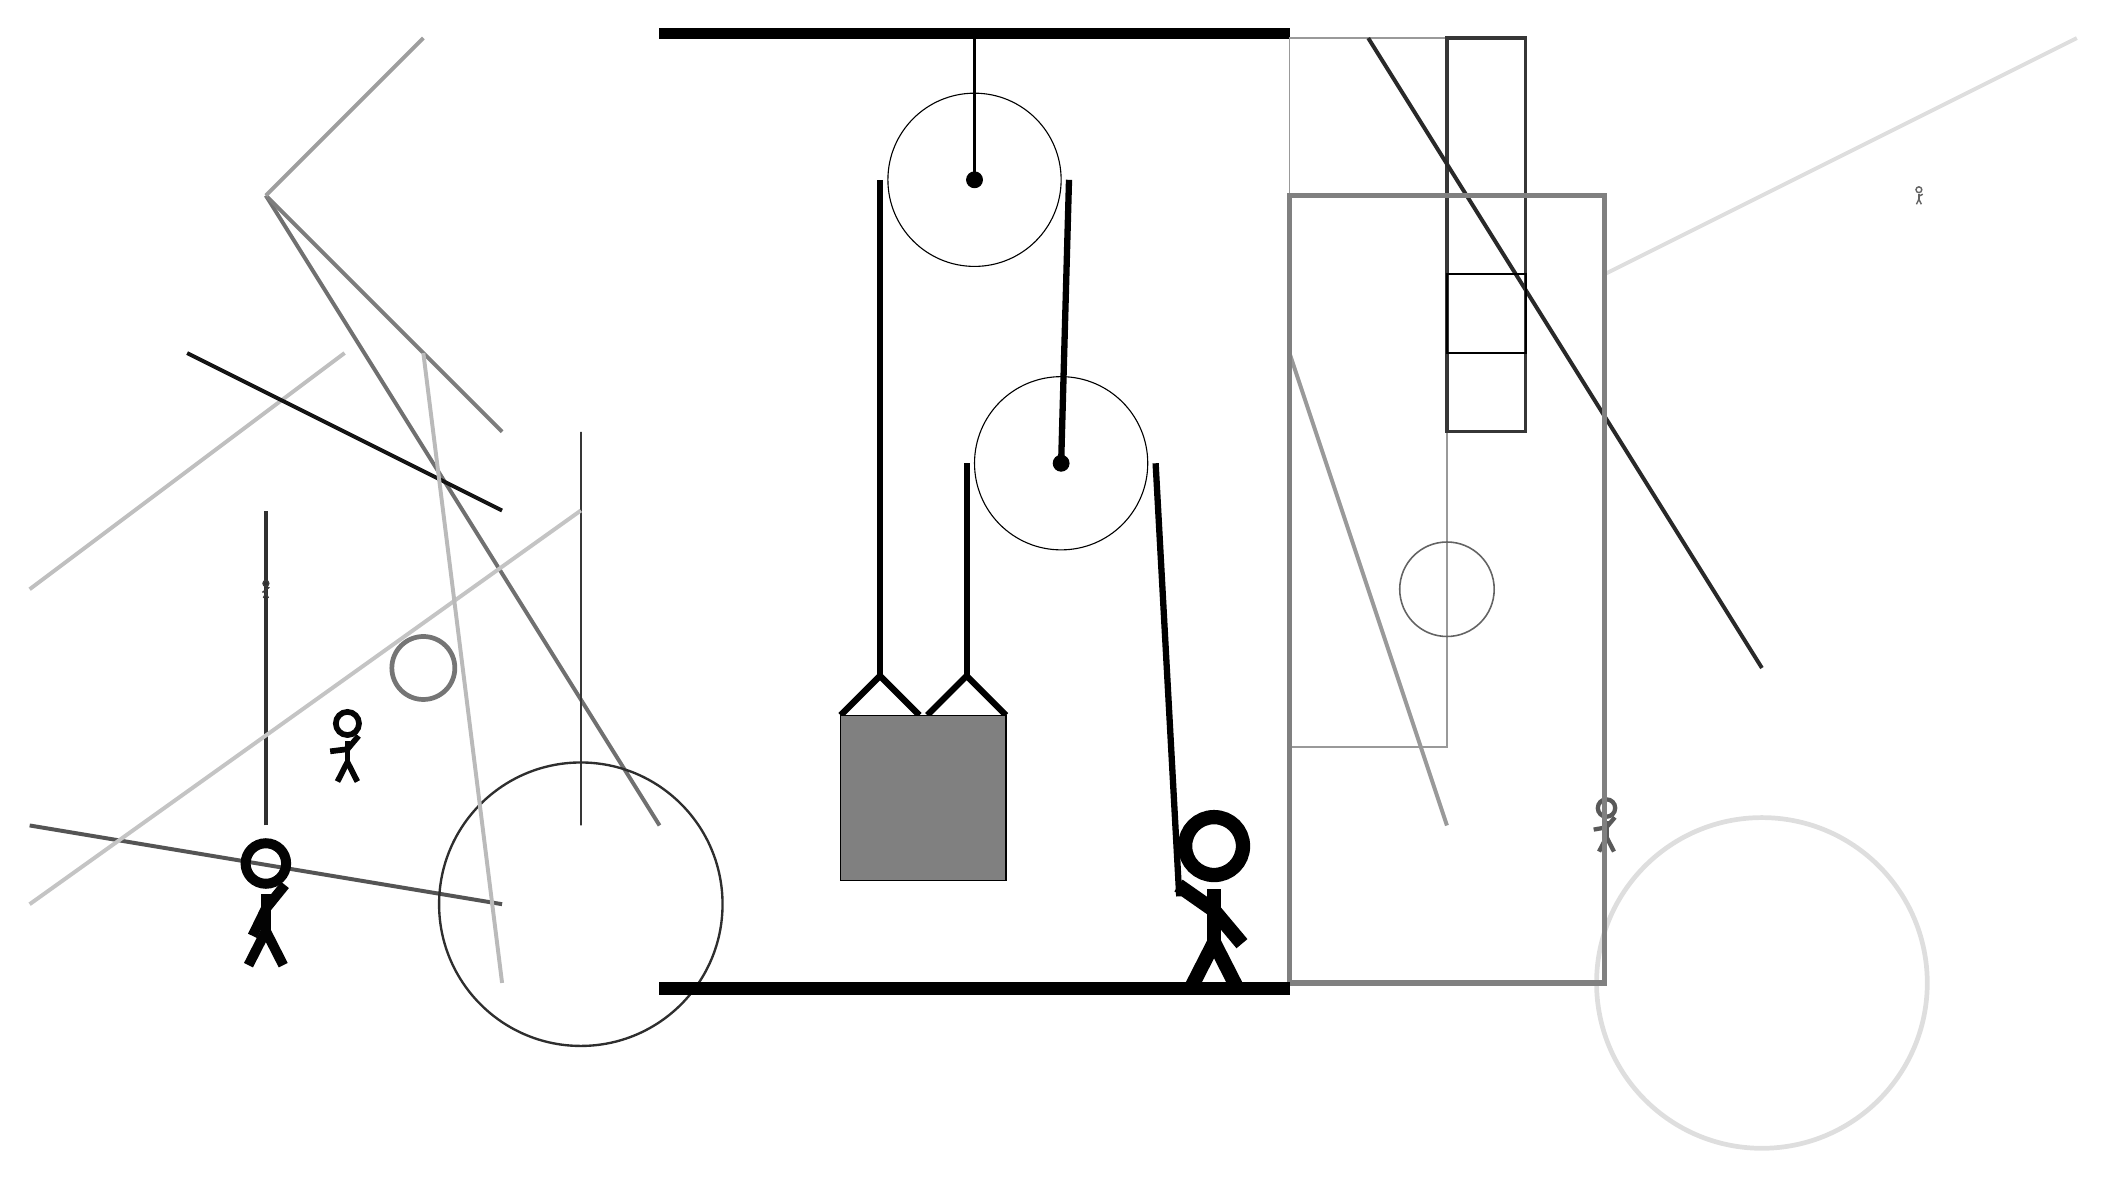
\begin{tikzpicture}
			%%%%% START %%%%%
			
			\draw[fill=black] (-2, 9) rectangle (6, 9.125);
			
			\draw (2, 7.2) circle (1.1);
			\draw[fill=black] (2, 7.2) circle (0.1);
			\draw[thick] (2, 7.2) -- (2, 9);
			
			\draw (3.1, 3.6) circle (1.1);
			\draw[fill=black] (3.1, 3.6) circle (0.1);
			
			\draw[line width=0.2mm, color=black!40] (8, 0) rectangle (6, 9);
			
			\draw[line width=0.5mm, color=black!56](-2, -1) -- (-7, 7);
			\node[line width=0.7mm, color=black!98] at (-6, 0) {\Strichmaxerl[4][7][50]};
			\draw[line width=0.5mm, color=black!25](-6, 5) -- (-10, 2);
			\draw[line width=0.5mm, color=black!67](-4, -2) -- (-10, -1);
			\draw[line width=0.3mm, color=black!79] (-3, -1) rectangle (-3, 4);
			\draw[line width=0.5mm, color=black!81](-7, -1) -- (-7, 3);
			\draw[line width=0.5mm, color=black!92](-4, 3) -- (-8, 5);
			\draw[line width=0.5mm, color=black!40](8, -1) -- (6, 5);
			\draw[line width=0.5mm, color=black!13](10, 6) -- (16, 9);
			\draw [line width=0.6mm, color=black!54](-5, 1) circle (0.4);
			\draw[line width=0.4mm, color=black!79] (8, 4) rectangle (9, 9);
			\draw[line width=0.5mm, color=black!51](-7, 7) -- (-4, 4);
			
			\draw[line width=0.5mm, color=black!23](-3, 3) -- (-10, -2);
			\draw [line width=0.3mm, color=black!82](-3, -2) circle (1.8);
			\node[line width=0.6mm, color=black!99] at (-7, -2) {\Strichmaxerl[7][64][51]};
			\draw[line width=0.5mm, color=black!84](7, 9) -- (12, 1);
			\node[line width=0.5mm, color=black!65] at (10, -1) {\Strichmaxerl[3][10][50]};
			\node[line width=0.5mm, color=black!77] at (-7, 2) {\Strichmaxerl[1][36][38]};
			\draw [line width=0.6mm, color=black!13](12, -3) circle (2.1);
			\node[line width=0.2mm, color=black!61] at (14, 7) {\Strichmaxerl[1][86][26]};
			
			\draw[line width=0.5mm, color=black!38](-7, 7) -- (-5, 9);
			\draw[line width=0.2mm, color=black!100] (8, 6) rectangle (9, 5);
			\draw [line width=0.2mm, color=black!61](8, 2) circle (0.6);
			\draw[line width=0.5mm, color=black!27](-4, -3) -- (-5, 5);
			\draw[line width=0.7mm, color=black!50] (6, -3) rectangle (10, 7);
			
			\draw[line width = 0.8mm]  (0.3, 0.4) -- (0.8, 0.9) -- (1.3, 0.4);
			\draw[line width = 0.8mm]  (1.4, 0.4) -- (1.9, 0.9) -- (2.4, 0.4);
			\draw[fill=black!50] (0.3, 0.4) rectangle (2.4, -1.7);
			
			\draw[line width = 0.8mm] (0.8, 7.2) -- (0.8, 0.9);
			\centerarc[line width = 0.8mm](2, 7.2)(0:180:1.2000000000000002);
			\draw[line width = 0.8mm] (3.2, 7.2) -- (3.1, 3.6);
			\draw[line width = 0.8mm] (1.9, 3.6) -- (1.9, 0.9);
			\centerarc[line width = 0.8mm](3.1, 3.6)(0:180:1.2000000000000002);
			\draw[line width = 0.8mm] (4.3, 3.6) -- (4.6, -1.9);
			
			\node at (5, -2) {\Strichmaxerl[10][-35][-50]};
			
			\draw[fill=black] (-2, -3) rectangle (6, -3.15);
			
			%%%%% END %%%%%
		\end{tikzpicture}
	\end{figure}	
\end{document}